% Created 2023-06-05 Mon 18:33
% Intended LaTeX compiler: pdflatex

\documentclass{revtex4-2}
\usepackage{siunitx}
\usepackage{graphicx}
\usepackage{amsmath}
\usepackage{tikz}
\usetikzlibrary{shapes,arrows,calc,positioning,backgrounds,fit}





\begin{document}



\title{Analysis of Niobium Electropolishing Using a Generalized Distribution of Relaxation Times Method}
\author{Eric Viklund}%
\email{ericviklund2023@u.northwestern.edu}
\affiliation{Department of Materials Science and Engineering, Northwestern University}%
\affiliation{Fermi National Accelerator Laboratory}%
\author{Vijay Chouhan}%
\affiliation{Fermi National Accelerator Laboratory}%
\author{Tim Ring}%
\affiliation{Fermi National Accelerator Laboratory}%
\author{Davida Smith}%
\affiliation{Fermi National Accelerator Laboratory}%
\author{David N. Seidman}%
\affiliation{Department of Materials Science and Engineering, Northwestern University}%
\author{Sam Posen}%
\affiliation{Fermi National Accelerator Laboratory}%
\date{\today}

\begin{abstract}
  Using electrochemical impedance spectroscopy, we have devised a method of sensing the microscopic surface conditions on the surface of niobium as it is undergoing an electrochemical polishing (EP) treatment. The method uses electrochemical impedance spectroscopy (EIS) to gather information on the surface state of the electrode without disrupting the polishing reaction. The EIS data is analyzed using a so-called distribution of relaxation times (DRT) method. Using DRT, the EIS data can be deconvolved into discrete relaxation time peaks without any apriori knowledge of the electrode dynamics. By analyzing the relaxation time peaks, we are able to distinguish two distinct modes of the EP reaction. As the polishing voltage is increased, the electrode transitions from the low voltage EP mode, characterized by a single relaxation time peaks, to the high voltage EP mode, characterized by two relaxation time peaks. We theorize that this second peak is caused by the formation of an oxide layer on the electrode. We also find that this oxide induced peak transitions from to a negative relaxation time, which is indicative of a blocking electrode process. By analyzing EPed samples, we show that samples polished in the low voltage mode have significantly higher surface roughness due to grain etching and faceting. We find that the surface roughness of the samples only improves when the oxide film peak is present and in the negative relaxation time region. This shows that EIS combined with DRT analysis can be used to predict etching on EPed Nb. This method can also be performed before or during the EP, which could allow for adjustment of polishing parameters to guarantee a smooth cavity surface finish.
\end{abstract}

\maketitle


\section{Introduction}
\label{sec:org5ef967f}
Electropolishing (EP) is commonly the method of choice to polish Nb superconducting radiofrequency (SRF) cavities. EP is an electrochemical polishing method using an HF containing electrolyte to dissolve the surface of the Nb under an applied votage. In ideal conditions, EP can acheive nanometer scale surface roughness. However, defects such as etching and pitting can sometimes occur especially when polishing larger, \qty{650}{\mega\hertz} cavities. One of the main causes of these defects has been shown to be insufficient voltage applied to the cavity during EP.\cite{chouhan2022study,viklund2022studies,chouhan2023electropolishing} To better understand why this is the case, we utilize a technique known as electrochemical impedance spectroscopy (EIS) to investigate the surface chemistry of Nb in the HF electrolyte.

EIS has been used to study the chemistry of niobium EP previously.\cite{cattarin2002nb,Tian_2008, tian2008novel, ranjith2018anodic} However, these studies only provide a basic analysis of the chemistry and rely on pre-supposed equivalent circuits to explain the measured impedance spectrum.

The goal of this study is to utilize EIS measurements to find the chemical mechanism behind the etching phenomenon without making apriori assumptions such as relying on a circuit model. To accomplish this, we use a model-free method of analyzing the EIS spectrum called distribution of relaxation times (DRT) analysis.\cite{10.1063/1.1745355, wan2015influence, ZHANG2015464} DRT analysis is used to extract the relaxation times of the chemical processes occuring on the electrode without the use of an equivalent circuit model. This method has been used to characterize a wide range of electrochemical systems such as fuel cells,\cite{Sonn_2008, schichlein2002deconvolution, Leonide_2008} batteries,\cite{SCHMIDT201370, batteries5020043, SONI202297} and supercapacitors.\cite{HELSETH2019100912} We  In section \ref{sec:org7d749e2} we show that these relaxation times are equivalent to the eigenvalues of the linearized electrochemical system dynamics. With this new insigt we generalize the DRT method to negative eigenvalues which correspond to unstable system dynamics, which is a necessary step for understanding the impedance characteristics of Nb EP.

Using this generalized DRT method, we are able to observe the formation of an NbO and an Nb\textsubscript{2}O\textsubscript{5} layer on the Nb electrode as the polishing voltage is increased. The formation of the Nb\textsubscript{2}O\textsubscript{5} oxide also corresponds with a reduction in surface etching indicating that the formation of this oxide layer is necessary to acheive good polishing.


\section{Experimental}
\label{sec:orgb71f960}

The electrolyte used for this experiment is composed of a 9:1 ratio of 98\% by volume sulfuric acid and 70\% by volume hydroflouric acid. A strip of Nb foil was prepared by cleaning with alcohol. Approximately \qty{8.4}{\centi\meter\squared} surface area of the strip was exposed to the electrolyte. A Nb wire was used as a reference electrode, since it is resistant to the EP electrolyte. The counter electrode is an aluminum rod. The temperature of the electrolyte was held at \qty{21}{\celsius} using an aluminum cooling coil immersed in the electrolyte. The EIS measurements were performed using a BioLogic VSP-300 potentiostat over a frequency range of \qtyrange{0.5}{2e5}{\hertz}. The EIS measurement was repeated for polishing voltages ranging from \qtyrange{0.5}{0.9}{\volt} measured versus the open circuit potential.

A series of Nb samples were electropolished using voltages ranging from \qtyrange{0.5}{1.2}{\volt} to determine the effect of the polishing voltage on the surface finish of the Nb. To remove any initial surface roughness from the samples a standard EP treatment was applied. \qty{10}{\micro\meter} of material was removed at a voltage of \qty{16}{\volt} creating a smooth surface finish. Then, \qty{5}{\micro\meter} of material was removed from each sample at lower voltages. To measure the surface finish after the low voltage polishing we use a Keyence VX-K 3000 confocal laser microscope to measure the 2D surface profile of the samples.



\section{Results}
\label{sec:org4a45003}

EIS measurements reveal a complex evolution of the surface chemistry as the polishing voltage is increased through the \qtyrange{0.5}{1.2}{\volt} range. As shown in figure~\ref{fig:nyquistplot}, at \qty{0.5}{\volt} the system exhibits a single capacitive impedance loop. This is most likely caused by the polarization of the electrode caused by the formation of an electrical double-layer.\cite{eliaz2018physical} At these low voltages, the reaction is charge transfer limited, the transfer of charged ions from the electrolyte to the Nb surface through the double-layer to oxidize the surface.

When the voltage is increased, two new features appear, an inductive impedance loop at mid-frequencies and a second capacitive impedance loop at low frequencies. This low frequency loop is caused by the formation of an oxide film and depletion of the HF near the electrode surface. This limits the current through the electrode at higher voltages. When the voltage is increased from \qty{0.78}{\volt} to \qty{0.86}{\volt} the direction of the low frequency loop changes from counter-clockwise to clockwise as shown in figure~\ref{fig:nyquistplot} indicating that the process dynamics have become unstable.

\begin{figure}[t]
  
  
\includegraphics[width=\textwidth]{../figures/nyquist.png}
  \caption{The complex impedance of Nb. Each plot shows the different regimes of electropolishing at low voltage. A one capacitive loop, B two capacitive loops, C capacitive, inductive, and capacitive loops, D capacitive, inductive, and capacitive loop with a negative resistance. The arrows indicate the direction of increasing frequency.}
  \label{fig:nyquistplot}
\end{figure}


\begin{figure}[t]
    
    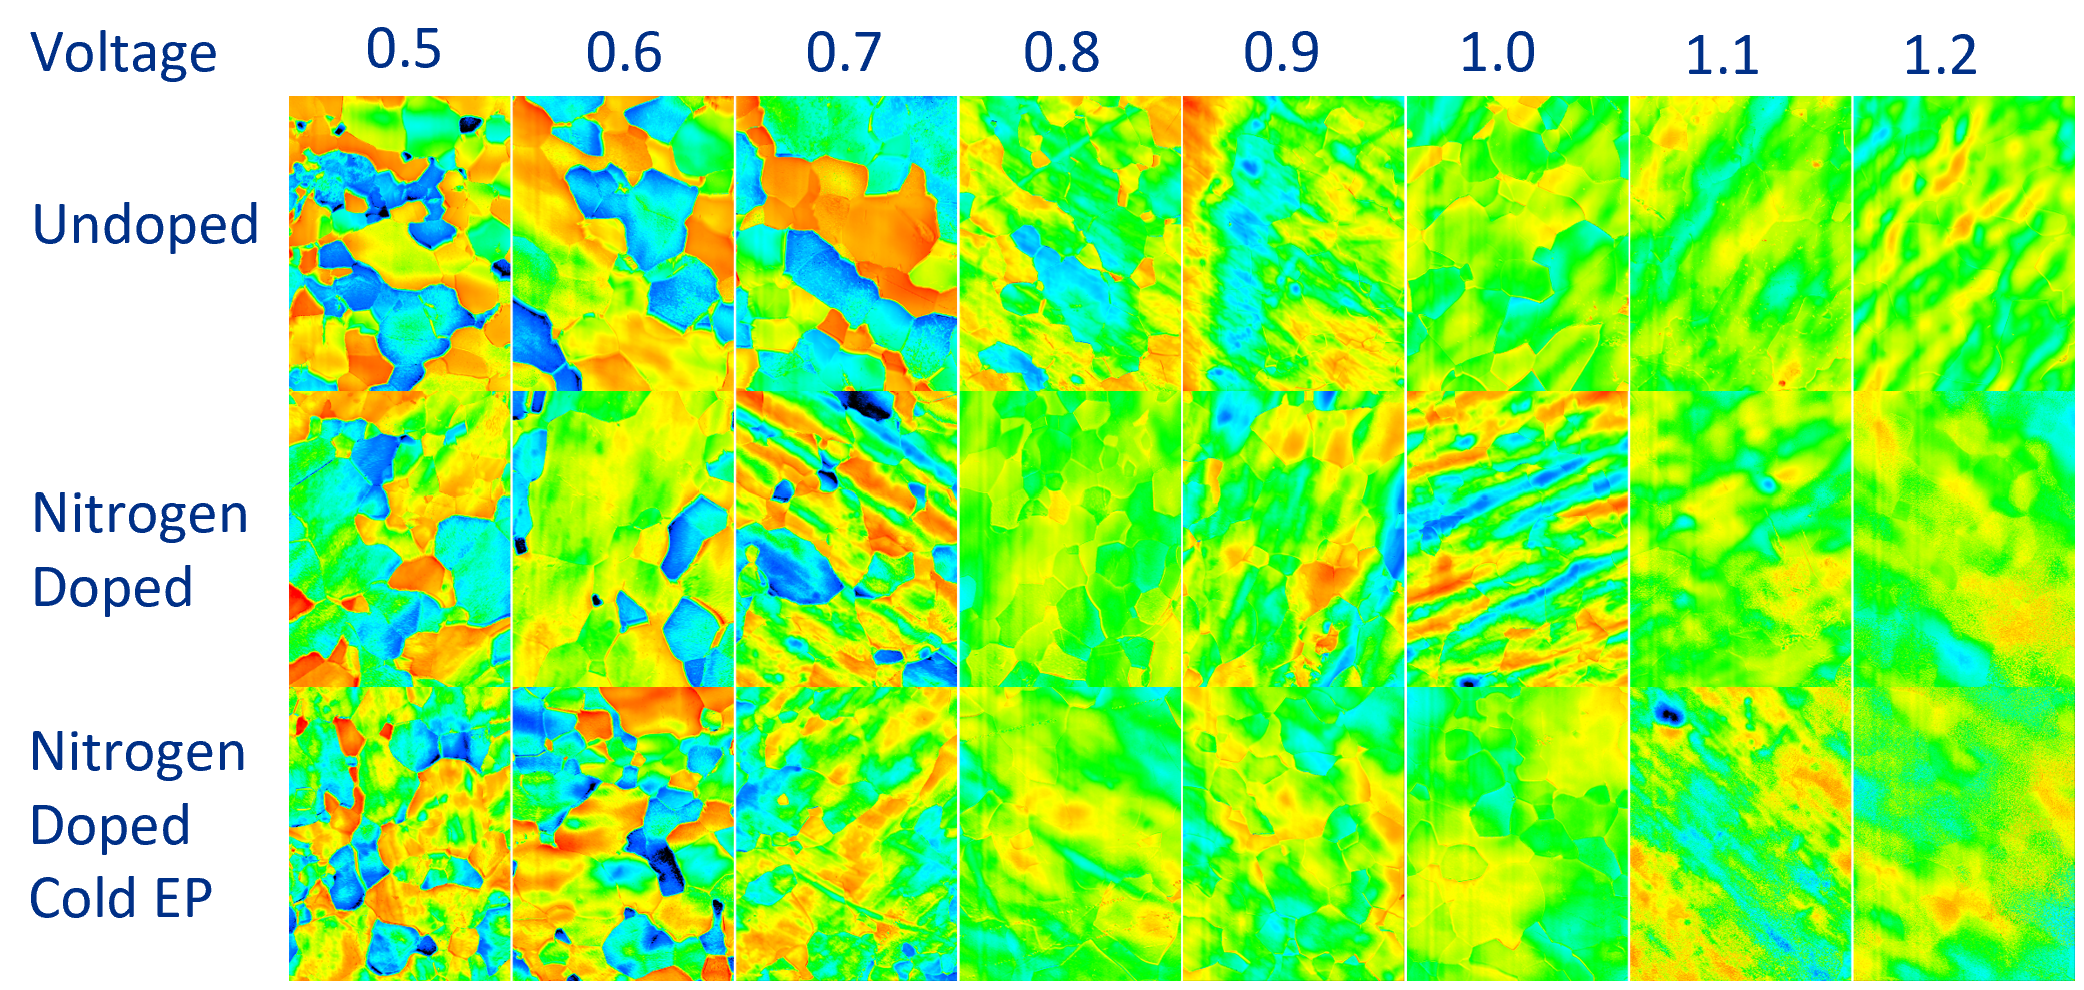
\includegraphics[width=\textwidth]{../figures/surface_maps.png}
    \caption{The surface height maps of Nb samples electropolished at different voltages and temperatures.}
    \label{fig:surface_maps}
\end{figure}





\section{Generalized Distribution of Relaxation Times}
\label{sec:org7d749e2}

As shown previously, the impedance spectrum is related to the eigenvalues of the electrochemical system's linearized dynamics.\cite{wu1998investigation, wu1999general} To calculate these eigenvalues from the experimental EIS measurements, we use the distribution of relaxation times (DRT) method. DRT is a flexible and general method that can be used to model impedance spectra without the use of an equivalent circuit model. The benefit of this method is that it does not require a presupposed circuit model, which may not be correct or have any physical meaning. The DRT method also allows for a linear fitting algorithm to be used instead of a non-linear one as shown in section~\ref{sec:sup}.

DRT analysis is typically based on an assumption that the electrode reaction can be modeled by a series of voigt circuits, a resistor and a capacitor connected in parallel. The electrode is simulated as a string of circuit elements consisting of infinitesimal voigt elements which can describe arbitrary capacitive impedance spectra. The impedance of Nb EP exhibits characteristics that cannot be described using only resistors and capacitors, the mid-frequency imductive impedance loop and the low-frequency unstable impedance loop. Therefore, it is necessary to generalize the DRT method to include these features.

We can express the impedance of the system as an integral equation where $G$ is the relaxation time distribution, $\omega_0$ is the inverse of the relaxation time also known as the natural frequency.

\begin{flalign}
  Z_{gDRT}\left(j \omega\right) &= \int_{-\infty}^{\infty} \frac{G\left(\omega_0\right) d\omega_0}{1 + j\frac{\omega}{\omega_0}} \label{eq:gDRT}
\end{flalign}

It was previously shown that the impedance of a linear system with first order dynamics can be written as a sum of the impedance contribution from each of the system's eigenvalues. The previous integral equation can be reduced to this form if $G$ is a sum of Dirac delta functions.

\begin{flalign}
  G\left(\omega_0\right) &= \sum_{n=1}^{N}\frac{\Omega_i}{\omega_0}\delta\left(\omega_0+\lambda_i\right)\\
  Z_{gDRT}\left(j \omega\right) &= \int_{-\infty}^{\infty} \frac{\sum_{n=1}^{N}\frac{\Omega_i}{\omega_0}\delta\left(\omega_0+\lambda_i\right) d\omega_0}{1 + j\frac{\omega}{\omega_0}}\\
  Z_{gDRT}\left(j \omega\right) &= \sum_{n=1}^{N} \frac{\Omega_{i}}{j \omega - \lambda_{i}} \\
\end{flalign}

From this we can see that $G$ and $\omega_0$ are related to $\Omega$ and $\lambda$. For a real measurement, the peaks in the DRT will not be perfect delta functions, but instead will have some width due to measurement noise and the finite number of data points. For a peak centered on the frequency $\omega_i$, we can approximate $\Omega_i$ and $\lambda_i$ as

\begin{flalign}
  \Omega_i &\approx \int_{\omega_i}\omega_0 G\left(\omega_0\right) d\omega_0\\
  \lambda_i &= -\omega_i \\
\end{flalign}

The eigenvalues of the electrochemical system are therefore related to the peaks in the distribution time. The frequency of those peaks gives the eigenvalues of the system. Positive frequencies correspond to stable eigenvalues, $\lambda < 0$, and negative frequencies correspond to unstable eigenvalues, $\lambda > 0$. The area under each peak is proprtional to the contribution of each eigenvalue to the total impedance spectrum. DRT can in principle also model higher order impedance spectra, which are present in systems with complex or repeated eigenvalues. However, in this case the DRT will not take the form of delta functions. A non-homogeneous electrode surface may also affect the DRT. Rather than a single eigenvalue, a non-homogeneous electrode will have a distribution of eigenvalues caused by the varying surface conditions. This effect would cause the sharp peaks of the DRT to become more broad.


\section{Distribution of Relaxation Times of Niobium Electropolishing}



\begin{figure}[t]
  
  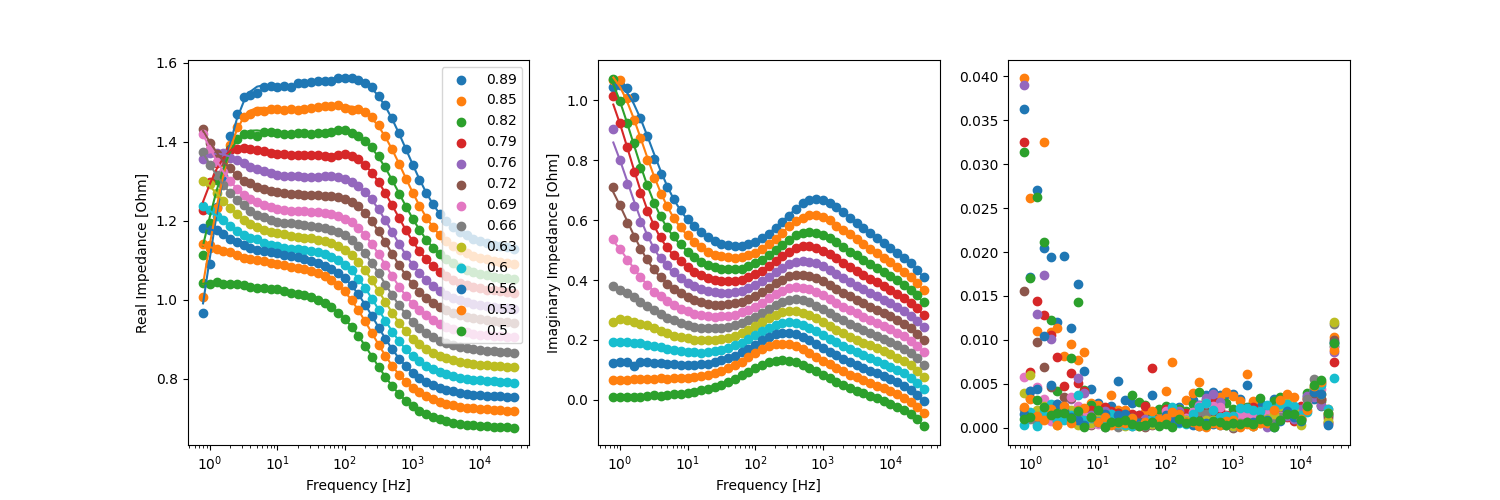
\includegraphics[width=\textwidth]{../figures/bodeplot.png}
  \caption{The complex impedance of Nb in electropolishing electrolyte measured using EIS. Each curve is offset from zero. The solid line shows the simulated impedance spectrum from the DRT model.}
  \label{fig:bodeplot}
\end{figure}

\begin{figure}[t]
  
  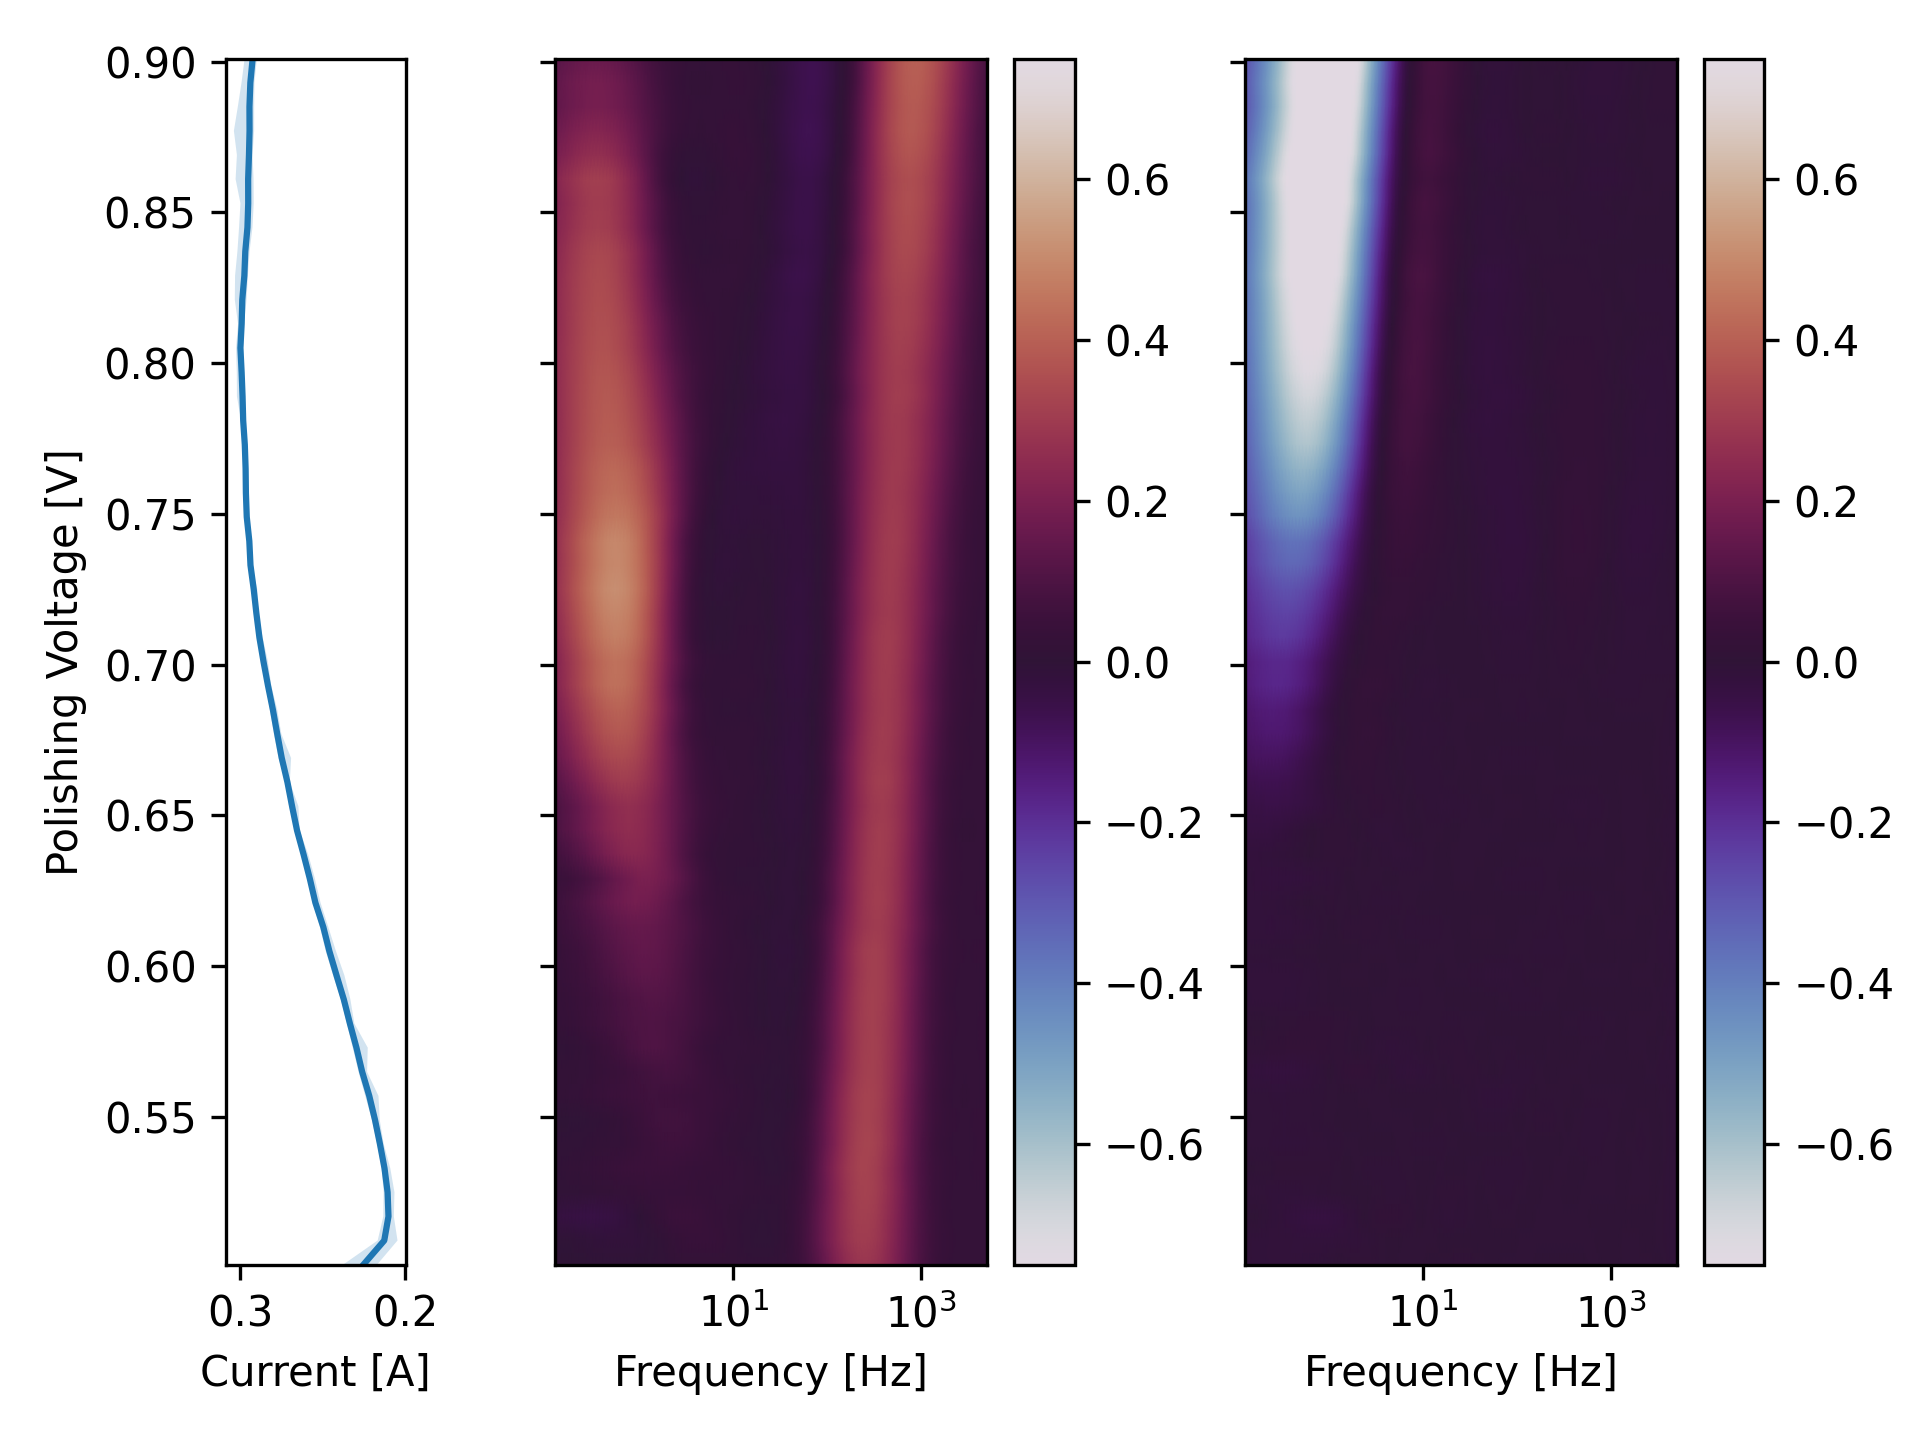
\includegraphics[width=\textwidth]{../figures/gamma.png}  
  \caption{The Distribution of relaxation times calculated from the EIS impedance data for each of the measured potentials. The current-voltage curve is shown in the graph on the left. The left DRT plot shows eigenvalues that are less than zero, which correspond to stable eigenvalues. The right DRT plot shows eigenvalues that are greater than zero, which correspond to unstable eigenvalues.}
  \label{fig:gamma}
\end{figure}

Using the generalized DRT method, we are able to fit the Nb impedance spectrum across all frequencies including the inductive mid-frequency loop and the low frequency loop as seen in figure \ref{fig:bodeplot}. From figure \ref{fig:gamma} we can see that there are three prominent peaks in the DRT. The peak centered around \qtyrange{100}{1000}{\hertz} corresponds to the electric double layer capacitance. This is clear because the peak exists at all voltages including low voltage. The center of this peak shifts to the right linearly with the polishing voltage. The frequency is plotted on a logarithmic scale, which shows that the relaxation time of the electric double layer follows an Arrhenius type relation.

The two other peaks centered around \qty{10}{\hertz}, one with a stable eigenvalue and one with an unstable eigenvalue. These peaks likely correspond to niobium oxidation reactions. The stable peak with a maximum around \qtyrange{0.7}{0.75}{\volt} is caused by the oxidation of Nb to NbO, while the unstable peak with a maximum at \qtyrange{0.8}{0.9}{\volt} is caused by the oxidation of NbO to Nb\textsubscript{2}O\textsubscript{5}. This can be verified by XPS measurements of Nb exposed to HF electrolytes in the active and passive regimes.\cite{ranjith2018anodic} The NbO peak first appears in the active region of the current voltage curve and reaches a maximum when the Nb transitions to the passive region. The Nb\textsubscript{2}O\textsubscript{5} peak appears in the active to passive transition region and grows larger in the passive region. This indicates that the Nb surface is becoming more oxidized as the polishing voltage increases and more of the surface is being covered by Nb\textsubscript{2}O\textsubscript{5}. 






\section{Discussion}

We propose a possible two step oxidation reaction mechanism to explain this behavior. At low voltages, the Nb is oxidized to the $Nb^{2+}$ oxidation state creating NbO. This NbO is immediately dissolved by HF since the reaction rate is limited by the oxidation step at low voltage. The rate of oxidation is dependent on the Nb grain orientation which leads to the observed grain etching phenomenon at low voltage. Once the voltage is increased, the oxidation rate is large enough for a thin layer of NbO to form on the surface as shown by the first oxidation peak in the DRT. As the voltage increases further, the oxidation state of Nb gradually changes to $Nb^{5+}$ through the formation of Nb\textsubscript{2}O\textsubscript{5} as shown by the second oxidation peak in the DRT. A diagram of this reaction mechanism is shown in figure~\ref{fig:diagram}.




\begin{figure}[t]
  \centering
  
  

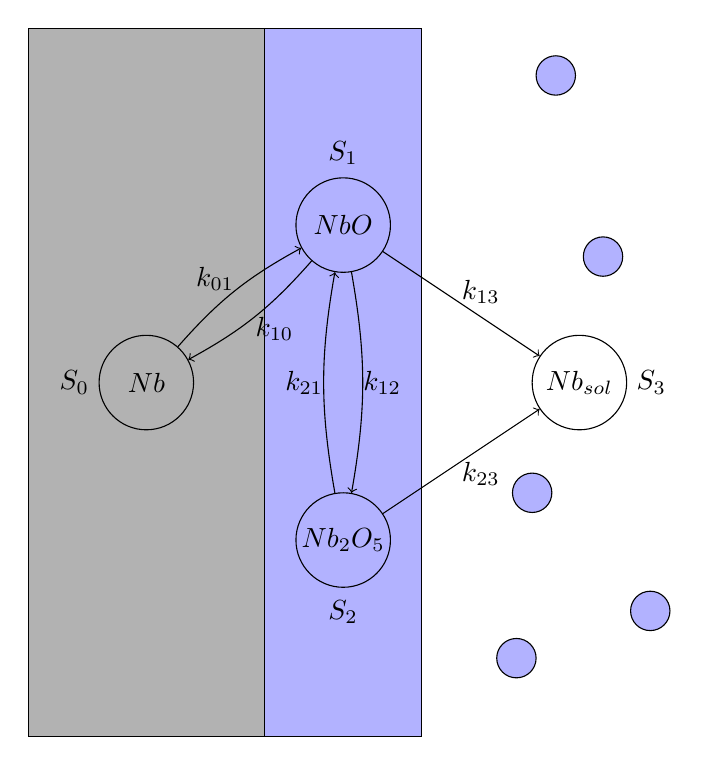
\begin{tikzpicture}[inner sep=0pt,minimum size=12mm,
                    every label/.style={minimum size=6mm}]
    \node at (-1.5, 0.0) (Nb)    [circle,draw,label=left:$S_0$]         {$Nb$};
    \node at ( 1.0, 2.0) (NbO)   [circle,draw,label=above:$S_1$]        {$NbO$}
        edge [->, bend left = 10]   node [auto, minimum size=1mm]       {$k_{10}$}  (Nb)
        edge [<-, bend right = 10]  node [auto, swap, minimum size=1mm] {$k_{01}$}  (Nb);
    \node at ( 1.0,-2.0) (Nb2O5) [circle,draw,label=below:$S_2$]        {$Nb_2O_5$}
        edge [->, bend left = 10]   node [auto, minimum size=1mm]       {$k_{21}$}  (NbO)
        edge [<-, bend right = 10]  node [auto, swap, minimum size=1mm] {$k_{12}$}  (NbO);
    \node at ( 4.0, 0.0) (Nbaq)  [circle,draw,label=right:$S_3$]        {$Nb_{sol}$}
        edge [<-]  node [auto, swap, minimum size=1mm]                  {$k_{13}$}  (NbO)
        edge [<-]  node [auto, minimum size=1mm]                        {$k_{23}$}  (Nb2O5);

    \draw [fill=blue!30] ( 3.7  , 3.9) circle (0.25);
    \draw [fill=blue!30] ( 4.3  , 1.6) circle (0.25);
    \draw [fill=blue!30] ( 3.4  , -1.4) circle (0.25);
    \draw [fill=blue!30] ( 4.9  , -2.9) circle (0.25);
    \draw [fill=blue!30] ( 3.2  , -3.5) circle (0.25);

    \begin{scope}[on background layer]
        \draw [fill=black!30] (-3  ,-4.5) rectangle ( 0  , 4.5);
        \draw [fill=blue!30]  ( 0  ,-4.5) rectangle ( 2  , 4.5);
    \end{scope}
\end{tikzpicture}


  \caption{Proposed mechanism for niobium electropolishing in HF containing electrolyte by a two step oxidation reaction.}
  \label{fig:diagram}
\end{figure}



Due to slight differences in the oxidation reaction activation energy across the surface, caused by differing grain orientations, surface defects, and the local curvature, the oxide forms preferentially in certain areas. The surface has a mixed oxide with a certain fraction covered by Nb\textsubscript{2}O\textsubscript{5}, NbO, and Nb. As the surface potential is increased a larger portion of the electrode is covered by Nb\textsubscript{2}O\textsubscript{5}. Once the entire surface is covered, the dissolution rate of the surface becomes homogeneous and polishing can occur. If the polishing voltage is not sufficiently high across the surface of the niobium, some areas will experience etching instead of polishing. This effect can be seen in \ref{fig:surface_maps}. On samples polished at low voltage, some of the grains have a facetted surface indicating that grain orientation effects are significant. This faceting disappears when the polishing voltage is above ~\qty{0.8}{\volt}. This effect coincides with the appearance of the Nb\textsubscript{2}O\textsubscript{5} oxidation peak in figure~\ref{fig:nyquistplot}, C.

Comparing figure \ref{fig:gamma} to the electropolished samples shown in figure \ref{fig:surface_maps} we can see that the appearance of the third peak coincides with a significant change in the surface of the electropolished niobium. The surface goes from an etched surface with facets and large grain boundary steps to a much more polished finish. We theorize that this transition is caused by the stabilization of the oxide film which occurs when the HF is depleted on the niobium electrode surface and the surface oxide transitions from a thin non-homogeneous layer to a thick homogeneous one. Since the oxide film is homogeneous, the effects of grain orientation on the dissolution reaction are eliminated. The result is a smoothing effect on the niobium. At polishing voltages below this critical voltage, the oxide film is too thin or does not cover the entire niobium surface, which leads to etching.

Compared to the small scale samples shown in this study, it is much more difficult to control the polishing voltage when eletcropolishing cavities. This is due to the much larger current and complex geometry of the cavity and cathode. Currently, cavity electropolishing machines do not employ a reference electrode and instead only set a fixed voltage between the anode and cathode. This means that cathode losses and ohmic losses in the electrolyte can significantly alter the polishing potential and even create a non-homogeneous potential distribution over the surface of the cavity. This is why etching can occur even when applying much higher potentials typically used during cavity EP.

To combat the uncertainty of electropolishing cavities it may be possible to apply EIS measurements in the production environment. This would allow for a live diagnostic of the polishing conditions inside the cavity without interfering with the regular EP workflow. This information can be used to tweak the EP parameters such as voltage and temperature to ensure that the cavity is in an optimal polishing regime. Using this technique it may be possible to electropolish more complex cavity geometries such as quarter-wave and half-wave geometries.



\section{Conclusion}
\label{sec:org57282ed}
In this study we have shown that the etching phenomenon seen in electropolished SRF cavities is caused by insufficient polishing voltage. Niobium polished below a critical voltage will experience etching whereas niobium polished above this voltage will experience smoothing. We theorize that the cause of this change in surface finish is a transition from a partially formed niobium oxide film to a fully formed, stable oxide film. This theory is evidenced by measurements of the niobium electropolishing impedance spectrum over a range of polishing voltages. The impedance spectrum indicates the presence of a blocking mechanism that limits the current. This blocking mechanism is most likely caused by the oxide film which forms when HF is depleted near the niobium surface and the oxidation rate exceeds the rate of dissolution by HF.


\section{Supplemental Information}
\label{sec:sup}

This Supplemental section will cover the mathematical process of calculating the generalized DRT from experimental measurements of the impedance spectrum. To find the DRT numerically, we must first discretize it using a finite set of basis functions which will approximate the continuous DRT. This is done by first transforming the problem into log coordinates. For a chosen basis function, the integral can then be calculated numerically and the problem is then transformed into a constrained linear regression problem.

\subsection{Discretizing the Integral of the Generalized DRT Function in Log Coordinates}

It is necessary to discretize the DRT in the log based coordinate system. It is typical to measure the impedance at frequencies spaced logarithmically to cover a wide frequency range. Therefore, it is also necessary to calculate the DRT in logarithmic coordinates. Otherwise, the computational accuracy will be too low at the low frequencies, or too high at the high frequencies. However, this is challenging when using the generalized DRT model, since the integral over $\omega_0$ in equation~\ref{eq:gDRT} spans both positive and negative values. To solve this problem we must separate the integral into the sum of two integrals each integrating over one half of the real axis. After a change of variables and reversing the direction of integration we can substitute $G\left(\omega_0\right)$ with a piece wise fit function $\gamma_{\pm}\left(\ln\omega_0\right)$.



\begin{flalign}
  Z_{gDRT} =& R_{s} + \int_{-\infty}^{0}\frac{G(\omega_0)d\omega_0}{1 + j \frac{\omega}{\omega_0}} + \int_{0}^{\infty}\frac{G(\omega_0)d\omega_0}{1 + j \frac{\omega}{\omega_0}}\\
  Z_{gDRT} =& R_{s} + \int_{0}^{\infty}\frac{G(\omega_0)d\omega_0}{1 + j \frac{\omega}{\omega_0}} + \frac{G(-\omega_0)d\omega_0}{1 - j \frac{\omega}{\omega_0}}\\
  G\left(\omega_0\right) d\omega_0 =& \begin{cases}
    \gamma_+\left(\ln\omega_0\right) d\ln\omega_0 & \omega_0 \ge 0 \\
    \gamma_-\left(\ln-\omega_0\right) d\ln\omega_0 & \omega_0 \le 0 \\
  \end{cases}\\
  Z_{gDRT} =& R_{s} + \int_{-\infty}^{\infty}\frac{\gamma_+\left(\ln\omega_0\right) d\ln\omega_0}{1 + j \frac{\omega}{\omega_0}} + \frac{\gamma_-\left(\ln\omega_0\right) d\ln\omega_0}{1 - j \frac{\omega}{\omega_0}}
\end{flalign}

To find the functions \(\gamma_{\pm}(\ln\omega_0)\) numerically we approximate them using a set of basis functions $\phi_n\left(\ln\omega_0\right)$.

\begin{flalign}
  \gamma_{\pm}(\ln\omega_0)&\approx\sum_{n=1}^{N}x^{\pm}_{n}\phi_{n}(\ln\omega_0)\\
  Z_{gDRT} =& R_{t} + \int_{-\infty}^{\infty}\sum_{n=1}^{N}\frac{x^{+}_{n}\phi_{n}(\ln\omega_0)d\ln\omega_0}{1 + j \frac{\omega}{\omega_0}} + \sum_{n=1}^{N}\frac{x^{-}_{n}\phi_{n}(\ln\omega_0)d\ln\omega_0}{1 - j \frac{\omega}{\omega_0}}
\end{flalign}

Using algebraic manipulation and a change of variables, the integral can be separated into a real part and an imaginary part.

\begin{flalign}
  x_n^{re} =& x_n^+ + x_n^-\\
  x_n^{im} =& x_n^+ - x_n^-\\
  Z_{gDRT} =& R_{s} + \sum_{n=1}^{N}x^{re}_{n} \int_{-\infty}^{\infty} \frac{\phi_{n}(\ln\omega_0)d\ln\omega_0}{1 + \left(\frac{\omega}{\omega_0}\right)^2} + j \sum_{n=1}^{N}x^{im}_{n} \int_{-\infty}^{\infty} \frac{\frac{\omega}{\omega_0}\phi_{n}(\ln\omega_0)d\ln\omega_0}{1 + \left(\frac{\omega}{\omega_0}\right)^2}
\end{flalign}

The impedance at a frequency $\omega = \omega_m$ is a linear function of the values of $x^{re}_n$ and $x^{im}_n$.

\begin{flalign} 
  Z_{gDRT}\left(j \omega_m\right) =& R_{s} + \sum_{n=1}^{N} x^{re}_{n} A^{re}_{n,m} + \sum_{n=1}^{N} x^{im}_{n} A^{im}_{n,m}\\
  A^{re}_{n,m} =& \int_{-\infty}^{\infty} \frac{\phi_{n}(\ln\omega_0)d\ln\omega_0}{1 + \left(\frac{\omega_m}{\omega_0}\right)^2}\label{eq:A_re}\\
  A^{im}_{n,m} =& \int_{-\infty}^{\infty} \frac{\frac{\omega_m}{\omega_0}\phi_{n}(\ln\omega_0)d\ln\omega_0}{1 + \left(\frac{\omega_m}{\omega_0}\right)^2}\label{eq:A_im}
\end{flalign}

Given a set of M experimentally measured impedance data points, $\mathbf{Z_{exp}} = \left[Z_1, \ldots, Z_M\right]$ at frequencies $\mathbf{\omega} = \left[\omega_1, \ldots, \omega_M\right]$ we can find the values of $x^{re}_n$ and $x^{im}_n$ using linear regression.

\begin{flalign}
  \min_{\mathbf{x^{re}},\mathbf{x^{im}}}\lVert\mathbf{Z_{gDRT}}-\mathbf{Z_{exp}}\rVert = \min_{\mathbf{x^{re}},\mathbf{x^{im}}}\left(\lVert \mathbf{x^{re}} \mathbf{A^{re}} - Re\left(\mathbf{Z_{exp}}\right) \rVert + \lVert \mathbf{x^{im}} \mathbf{A^{im}} - Im\left(\mathbf{Z_{exp}}\right) \rVert \right)\label{eq:Zmatrix}
\end{flalign}

\subsection{Normalization}

When finding the DRT function from experimental data, a normalization method is required to prevent overfitting. In this study we use a modified Tikhonov regularization, based on the work of Wan, et. al.~\cite{wan2015influence}, that penalizes the derivatives of the DRT function. This has the effect of smoothing the function and eliminating oscillations caused by overfitting. With the regularization term added the objective becomes to minimize the residuals and the normalization term together. 

\begin{flalign}
  \min_{\mathbf{x^{re}},\mathbf{x^{im}}}\left(\lVert \mathbf{x^{re}} \mathbf{A^{re}} - Re\left(\mathbf{Z_{exp}}\right) \rVert + \lVert \mathbf{x^{im}} \mathbf{A^{im}} - Im\left(\mathbf{Z_{exp}}\right) \rVert + \mathbf{x^{re} M x^{re}}^T + \mathbf{x^{im} M x^{im}}^T \right)
\end{flalign}

The matrix $\mathbf{M}$ is calculated by integrating the square of the derivatives of the test functions, $\phi_n\left(\omega_0\right)$. Calculating the zeroth derivative, i.e. the function itself, is equivalent to standard Tikhonov regularization. The strength of the regularization is controlled by multiplying by a constant $\lambda_k$, where $k$ is the k-th derivative of the test functions.

\begin{flalign}
  (\mathbf{M}_{k})_{n,m} =& \int_{-\infty}^{\infty} \frac{d^{k}\phi_{n}}{dln\tau^{k}} \frac{d^{k}\phi_{m}}{dln\tau^{k}} dln\tau\\
  \mathbf{M} =& \sum_{k=0}^{K}\lambda_{k}\mathbf{M}_{k}
\end{flalign}

The optimum values of \(\lambda_k\) are difficult to find mathematically, so values were manually adjusted up to $k=2$ to eliminate oscillations without sacrificing the accuracy of the fit. Mathematical heuristics such as the L-curve, cross-validation, Fourier transform\cite{BOUKAMP201712} or Bayesian methods\cite{ciucci2015analysis} can be used to more precisely optimize the regularization parameters.





\subsection{Basis Function}
\label{sec:org8198a5a}

The choice of basis function is quite arbitrary as long as the resulting function space is large enough to approximate the exact solution for the DRT function. However, in practice the basis function has a large impact on the number of parameters required and the level of regularization required. The basis function should also be relatively easy to compute using a computer to speed up the computation and the function should be differentiable so that the regularization matrix can be calculated. A natural choice is to use the log Gaussian, which has been shown to be effective at fitting the DRT function for several kinds of impedance systems\cite{wan2015influence}. These functions are gaussian functions in the log coordinates shifted by $\ln\left(\omega_n\right)$.

\begin{flalign}
  \phi_{n}(ln\omega) &= \frac{1}{\sigma\sqrt{2\pi}}e^{-\left(\frac{ln\omega-ln\omega_{n}}{\sigma\sqrt{2}}\right)^2}
\end{flalign}

Combining this test function with equation~\ref{eq:A_re} and \ref{eq:A_im} gives the following expressions for the matrices $A_{re}$ and $A_{im}$.

\begin{flalign}
  A^{re}_{n,m} =& \frac{1}{\sigma\sqrt{2\pi}} \int_{-\infty}^{\infty} \frac{e^{-\left(\frac{ln\omega_0-ln\omega_{n}}{\sigma\sqrt{2}}\right)^2} d\ln\omega_0}{1 + e^{2\left(\ln\omega_m - \ln\omega_0\right)}}\\
  A^{im}_{n,m} =& \frac{1}{\sigma\sqrt{2\pi}} \int_{-\infty}^{\infty} \frac{e^{\ln\omega_m-\ln\omega_0} e^{-\left(\frac{ln\omega_0-ln\omega_{n}}{\sigma\sqrt{2}}\right)^2} d\ln\omega_0}{1 + e^{2\left(\ln\omega_m - \ln\omega_0\right)}}
\end{flalign}

These integrals are calculated numerically and used to find the DRT.


\bibliography{generalized_DRT}


\end{document}